\definecolor{grayR}{rgb}{0.50, 0.50, 0.50}
\definecolor{grayB}{rgb}{0.10, 0.10, 0.10}
\definecolor{grayY}{rgb}{1.00, 1.00, 1.00}
%\def\myRed{red}
%\def\myBlue{blue}
%\def\myYellow{yellow}
\def\myRed{grayR}
\def\myBlue{grayB}
\def\myYellow{grayY}

% wellcolored
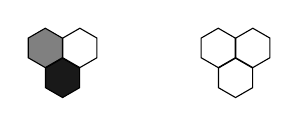
\begin{tikzpicture}[scale=0.25]
  %1段目
  \filldraw[fill=\myBlue,xshift={-25*5},yshift={25*sqrt(3)*3}] (0,0)--++(30:1)--++(90:1)--++(150:1)--++(210:1)--++(270:1)--cycle;
  \filldraw[fill=\myYellow,xshift={25*5},yshift={25*sqrt(3)*3}] (0,0)--++(30:1)--++(90:1)--++(150:1)--++(210:1)--++(270:1)--cycle;
  %0段目
  \filldraw[fill=\myYellow,xshift={-25*4},yshift={25*sqrt(3)*4}] (0,0)--++(30:1)--++(90:1)--++(150:1)--++(210:1)--++(270:1)--cycle;
  \filldraw[fill=\myRed,xshift={-25*6},yshift={25*sqrt(3)*4}] (0,0)--++(30:1)--++(90:1)--++(150:1)--++(210:1)--++(270:1)--cycle;
  \filldraw[fill=\myYellow,xshift={25*6},yshift={25*sqrt(3)*4}] (0,0)--++(30:1)--++(90:1)--++(150:1)--++(210:1)--++(270:1)--cycle;
  \filldraw[fill=\myYellow,xshift={25*4},yshift={25*sqrt(3)*4}] (0,0)--++(30:1)--++(90:1)--++(150:1)--++(210:1)--++(270:1)--cycle;
\end{tikzpicture}
